\documentclass{tufte-handout}
\usepackage{amsmath}
\pagestyle{empty}
\usepackage[utf8]{inputenc}
\usepackage{mathpazo}
\usepackage{microtype}

\usepackage{tikz}
\usetikzlibrary{matrix}
\usetikzlibrary{chains}
\usetikzlibrary{decorations}

\input{vc.tex}  % For version control


\title{Super Vector Mario!}
\author{Thore Husfeldt}
\date{\GITAuthorDate, rev. \GITAbrHash}

\begin{document}

\maketitle

\subsection{Description}
Find the fastest trace for super mario.

\begin{marginfigure}
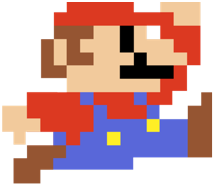
\includegraphics[width = 2in]{mario.png}
\end{marginfigure}

\subsection{Rules}
This games is a variant of \emph{Racetrack} or \emph{Vector Rally} that you may have played in school.\sidenote{You can read about the normal pen-and-pencil version of Vector Rally (with cars, not jumping plumbers) at Wikipedia's entry for {\bf Racetrack (game)}.}
The game is played on a grid, and the object is to get Mario (a jumping plumber) from a grid position marked ``S'' (for start) to a grid position marked ``F'' (for finish), in as few moves as possible.
Mario moves by jumping from one position to another, and he may never land on a gray square.
At any given time, Mario has a velocity $(\Delta x, \Delta y)$ in $x$- and $y$-directions.
In the beginning, he stands still, so his initial velocity is $(0,0)$.
Each turn, Mario moves from his current location $(x,y)$ to the new location $(x+\Delta x, y+\Delta y)$, provided the new position is not off-road.
In addition, Mario can increase or decrease his velocity in either direction by $1$.
For example, after the first step, Mario’s velocity might be any of $(-1,-1)$,  $(-1,0)$, $(-1,1)$, $(0,-1)$, $(0,0)$, $(0,1)$, $(1,-1)$, $(1,0)$, or $(1,1)$.
The goal is to get from any of the Ss to any of the Fs in as few moves as possible.
(Mario's speed when he reaches F is not important.)


\subsection{Example}

\begin{figure}
  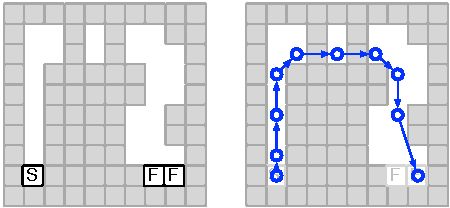
\includegraphics{racetrack.pdf}
  \caption{An input instance and a valid sequence of 10 moves.}
\end{figure}

Consider the input instance above.
The object is to get from the S square to any of the F squares (it does not matter which).
The offroad squares are grey.
Note that unlike what you may have played at school, the ``car'' (Mario) is allowed to ``jump''.\sidenote{This is because otherwise the exercises becomes much more difficult:  you'd have to calculate when ``arrows'' touch offroad corners, and then it’s suddenly an exercise in geometry, not graph algorithms}

\subsection{Requirements}

The data directory contains a number of test inputs with known optimal sequence lengths, your algorithm must work correctly on those.\sidenote{There can be many shortest paths, so it makes no sense to specify the positions on the path.}

\subsection{Deliverables}

\begin{enumerate}
  \item The source code for your implementation
  \item A report in PDF.
  Use the report skeleton in the {\tt doc directory}.
  \end{enumerate}

\subsection{Tips}

Yes, this is a graph connectivity exercise, and it can be solved with few lines of code.
The main difficulty is to find out what the graph is (what are the vertices, and how are they connected).
Solving an instance like {\tt twice-in.txt} by hand is probably helpful.

\end{document}
